\documentclass[a4paper]{report}

\usepackage{amsmath, amssymb}
\usepackage{multicol}
\setlength{\columnsep}{1cm}
\usepackage[margin=0.75in]{geometry}
\usepackage{graphicx}
\graphicspath{ {../../../Images/COIT11222/} }
\usepackage[breaklinks]{hyperref}
\usepackage{tikz}
\usepackage{stix}
\usepackage{ragged2e}

\begin{document}
	\begin{titlepage}
		\centering
		{\Huge \textsc{COIT11222}\par}
		\vspace{1cm}
		{\Large \textsc{The Weekly Notes}\par}
		\vspace{2.5cm}
		\vfill
		Authored by:\par
		Lachlan J. W. Wyer
		\vfill
		{\large Document Date: \par}
		\date{20/09/2025}
		{\large \today\par}
	\end{titlepage}
\begin{flushleft}
\begin{multicols}{2}
	\section*{Week 1 - Introduction:}
	\subsection*{Computer Architecture:}
	There are several components that make up the system.

	\subsubsection*{Central Processing Unit}
	The central processing unit, also known as the CPU, can be considered the brain of the computer. It carries out instructions \& calculations. The speed of the a CPU, measured in Hz, is the number of clock cycles per second. E.g. A 3GHz CPU can execute 3 billion cycles per second.

	\subsubsection*{Main Memory}
	This is the main memory of the CPU (e.g. RAM or CPU cache). It allows it to store items temporarily, making it a type of volatile memory. This is because the data is lost on power reset or the process completion.

	\subsection*{Secondary Memory}
	Unlike main memory, secondary memory is used to store long term data. It is slower then RAM/cache but contains the ability to store data through power loss and after process completion. Examples of secondary memory include flash storage, SSDs, HDDs, NVME \& USB.

	\subsection*{Input \& Output Devices}
	These devices have the ability to enable users to interact with a susystem. Like keyboards, mice, speakers, screens, microphone and touchpad.

	\subsection*{Network}
	Modern computers have network access which allow wireless connections. These can be local connection (LAN, bluetooth), or with the world (WAN).

	\subsection*{Communicating with the Computer:}
	There are two types of languages used to interface with a computer.
	\begin{enumerate}
		\item Machine Language: This is the lowest language that interfaces directly with the miroprocessor. Whilst it is the easiest to interface with the computer (Binary), it is not easily human readable.
		\item High-level Languages: These are the "normal" languages. Like python, rust, ruby, go, C/C++,C\#, QML or Java. These are normally quite human-readable, but require interpreters and compliation for the code to run on a computer. Needs to translate the code into Binary.
	\end{enumerate}

	\subsubsection*{Programs}
	For a computer to complete a complicated task, it can be brsoken down into a sequence of instructions. These instructions are written in a programming language are called a program.

	\subsubsection*{Interpretor vs Compiler}
	Interpretors take a program \& run it lin by line. It allows a universal way of running programs simply. Compared with a complier it runs through the whole program before running. This allows errors to be found before any parts are run. It also gives the opportunity for optimizations to happen locally for processes that do not need to run. Think Gentoo or PKGBUILD.h. There is a version of this called a hybrid model. They allow partial compilation can universal running.

	\subsection*{Debugging:}
	Programming can lead to errors, debugging is the process \& removal of such errors. There are three main types of errors:
	\begin{enumerate}
		\item Syntax Errors: Syntax within a program refers to its structure \& rules governing it. In python, it requires a line to be syntactically correct for it to run.
		\item Runtime Errors: RTEs occur when a program runs into unexpected problems during its execution. These errors can only be found once a program starts running, either through an interpretor or compilation.
		\item Semantic Errors: These errors occur when a program runs but the outupt is incorrect. Such as the logic of the being fundamentally wrong.
	\end{enumerate}
	
	\subsection*{Program Development:}
	\begin{enumerate}
		\item Analyze:
		\begin{itemize}
			\item Define the problem
			\item The desired output
			\item The inputs/data the program will use
			\item Determine anyn special use cases that program will have to deal with.
		\end{itemize}
		\item Design:
		\begin{itemize}
			\item Find the logical sequence of steps
			\item Develop an alogorithm (e.g. flowchart, table, psuedocode)
		\end{itemize}
		\item Algorithms:
		\begin{itemize}
			\item A step-by-step procedure of what is to be completed
			\item It is unambigous \& effective method that can be implemented in every type of programming language
			\item Needs to define clear I/O
			\item Be able to handle edge cases
			\item Of finite length \& terminate after a set of steps
		\end{itemize}
		\item Code:
		\begin{itemize}
			\item Translate the algorithm into a programminng language
		\end{itemize}
		\item Debug:
		\begin{itemize}
			\item Fix errors present within the code
			\item Find a way for the program to break
			\item Break the code, and remember that users are idiots and will test everything you did not think of
		\end{itemize}
		\item Documentation:
		\begin{itemize}
			\item Document what the code does. Allowing people to understand what each steg does and how it will complete it.
			\item Do not document obvious steps. E.g. \\
			\# Adds together 2 numbers
			$$z\;=\;x\;+\;y$$
		\end{itemize}
	\end{enumerate}

	\section*{Week 2 - Programming}
	\subsection*{Program Execution:}
	There are two views on a programs execution. The programmers view is where they can either write the program directly into the interpretor (one line at a time) or on a script (allows functions to be written). For running a script the order in the file is the way it will execute within the program. E.g. line numbers within a file. The complier and interpretors view is how is transcodes that file into byte code and routed into a PVM to translate it into machine code.

	\subsection*{Data Types:}
	There are several way of having data listed within python.
	\begin{center}
		\begin{tabular}{ |c|c| }
			\hline
			Type & Example \\
			\hline
			Text & str \\
			\hline
			Numeric & int, float, complex \\
			\hline
			Sequence & list, tuple, range\\
			\hline
			Mapping & dict \\
			\hline
			Set & set, frozenset \\
			\hline
			Boolean & bool \\
			\hline
			Binary & bytes, bytearray, memoryview \\
			\hline
			None & NoneType \\
			\hline
		\end{tabular}
	\end{center}
	It is important to note that when converting numbers to complex form in python, they cannot be easily converted back into int() or float(). Sequence types can be sequencetion. E.g. ['a', [1, 2, 3], 'c']. A descripition of the None Type is also required, as it defines a variable not referencing any memory location for a specific piece of data. To find the type a piece of data is, use the type() function.

	\subsection*{Variable:}
	A variable is a value stored in memory, and is assigned with the = operator, e.g. x = 2. Values in variables can change when re-assigned, even changing the type of data stored within it. When creating a variable it name, it cannot contain any of the key-words present within pythons global listings. The naming convention for variables in python is snake-case, e.g. variable\_name.
	\begin{center}
		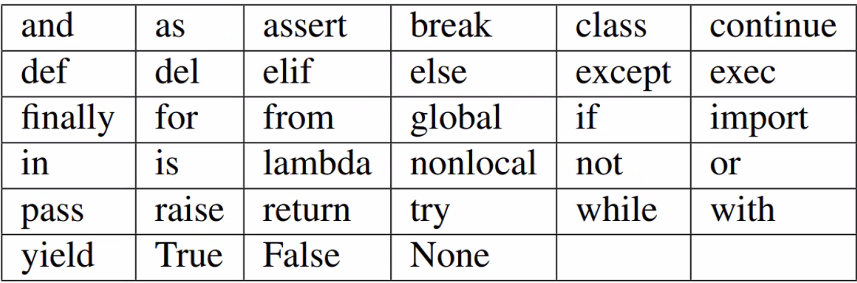
\includegraphics[scale=0.6]{no-variable-name.png}
	\end{center}
	\subsection*{Expressions:}
	An expression is a statement that changes a value and produces a result, e.g. x + 50 or x += 1 or 36. To do this there is usually an operator or command that is required. It python there are a number of different ones available. A point to note with floor division is that it rounds down to the nearest interger value. Like in normal maths, python follows BODMAS.
	\begin{center}
		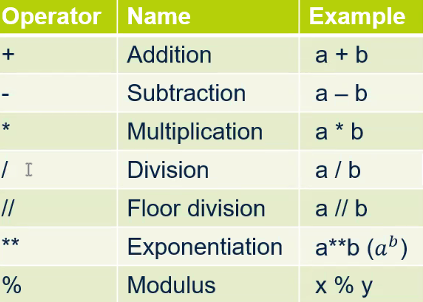
\includegraphics{operands-python.png}
	\end{center}
	\subsection*{Input:}
	Python uses the input function to parse in a user input into the program. It is important to note with this, that all values inputted into this are string values, even if technically thought to be another type. For example a user inputting a 5.5 is "5.5" rather than 5.5.

	\section*{Week 3 - Flowcharts and Psuedocode:}
	\subsection*{Flowcharts:}
	Using a variety of different of standardized symbols, the flowchart vizualizes the programs control/executional flow. With the symbols, the shape indicates the type of the operation that is occur (see image below). E.g. the parrallelogram indicating that an input or output, or the arrows denoting the path to take. The general consensus for a flowchart is to read them top to bottom.
	\begin{center}
		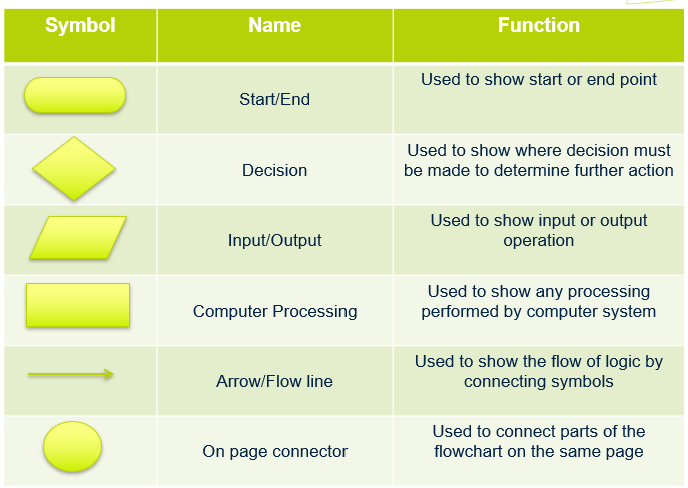
\includegraphics[scale=0.75]{flowchart-symbols.png}
	\end{center}

	\subsection*{Boolean Things:}
	\subsubsection*{Boolean Values:}
	These values are basics of every type of comparison within python. The two type a boolean value can be is True or False (must be with the capital).
	\subsubsection*{Boolean Expressions:}
	A boolean expression is an expression that evaluates an item to produce a result which is a boolean value. An example of this is the $==$ to check whether two values reference the same memory location. If they do (e.g. $6==6$) it will return True, else it would return false and continue to the next section within a program.

	\subsection*{Logical Operators:}
	Within python there are three types of logical operators.
	\begin{tabular}{|c|p{2.5cm}|p{2.5cm}|}
		\hline
		Operator & Descripition & Example \\
		\hline
		and & \RaggedRight Returns a True iff both operands on either side of the condition is True. If the first condition is false it will not test the second & \RaggedRight $x>0\;\text{and}\;x<10$ produces True only if x is greater then 0 and at the same time less than 10 \\
		\hline
		or & \RaggedRight Returns True if only one of the operands is True & \RaggedRight $n\%2==0\;\text{or}\;n\%3==0$ is True if either of the conditions is True. In this example it would return True if n is 2 or 9. \\
		\hline
		not & \RaggedRight Negates a boolean value & \RaggedRight not(x>y) is True if x>y is False. To sum it up, it just swap True<->False.\\
		\hline
	\end{tabular}
	\subsubsection*{Short  Circuit Evaluation:}
	This is the process python takes to evaluate variables. In a condition the expression to the left of the logical operator is evaluated first. To base this within the operators, for the or statement, if the first conditions is true it does not both to evaluate the second. Compared with the and, if the first one is false it does not check the second.
	\subsubsection*{if Statements:}
	An if statement is a construct that enables a program to specify alternative path flow for an execution. Such as when a user inputs something that is not a number, the program can explain that an error has occcured. In python the if statements go, if CONDITION: <return><tab>. Whilst technically not needed, as it can just run with on line, the PEP 8 standard would prefer it this to make the code more readable. Remember that if you would like it to run within the same block, use elif and else statements.
	\subsubsection*{match Statement:}
	The match statement is similar to an if statement, but it matches pattern against an expression. It can also contain the boolean expressions and if statements.

	\section*{Week 4 - Basics of Programming:}
	\subsection*{Data structures:}
	A data structure is a way of organizing and storing data with a system's memory. It's a like a container that holds different pieces of information in very specific and standardized data formats. Examples of data structures include lists, tuples, dictionaries, or arrays.
	
	\subsection*{Tuples:}
	Tuples are a way of storing data within an organized and immutable sense. E.g. once data has been entered into a tuple it cannot be changed. A tuple is created with the standard curved parantheses (). E.g. tuple = (1, 'abc'). To access the data within a tuple is to simply just an index. Indexing refers to a specific piece of data's reference within the tuple. E.g to access the 1, tuple[0]. It is crucial to note that indexing of all types starts from the value 0, and can be looped backwards through negative indexs. However it an index is larger then the largest value it will error out saying that x index does not exist.

	\subsection*{Functions:}
	Functions are a crucial part of any programming language. This is because it allows you to break down complex problems into smaller, and more manageable chunks of code. Functionas also allow a piece of code to repeat in variety of sections with different inputs. \\
	In python the keyword for functions is def functionName(parameters):<tab>. The function's name must be descripitive of what the function will achieve. In addition the parameters are an opitional addon to parse variable into it. To return any variables or strings or anything, a return <item> is used.
	\subsubsection*{Multiple Parameters:}
	There are two different ways of parsing in multiple parameters:
	\begin{enumerate}
		\item Positional Argument: This is where the variables being parsed in are order of the parameters in the function.
		\item Keyword Argument: Where the functions parameters are assigned like variables. This means that it does not have to be in order.
	\end{enumerate}
	The benefits of functions is that it allow repeated code to be reused, modularity and abstraction.
	\begin{itemize}
		\item Code Reusability: Allow blocks of code to be used in multiple places and even in different files. Reducing code duplication and leading to better code.
		\item Modularity: Allows the breaking down of complex logic into more manageable pieces. Each function only should do one thing, these can be combined into larger functions.
		\item Abstraction: Can break complex operations into simple function calls.
		\item Flexibility and Scalability: Functions can be modified, replaced or extended without affecting the rest of the code, as long as the function's interface remains the same.
		\item Debugging and Testing: By isolating specific logic, it makes it easier to identify and fix issues.
		\item Code organization and Readability: Function allow a developer to encapsulate specific logic, oragnize the code into smaller and manageable units. Making it easier to understand and maintain in future amounts.
	\end{itemize}

	\subsection*{Modules:}
	Modules in python is a seperate file containing python code that can be imported and used. Anything can be stored in a module, e.g. functions, classes, variables or combinations of all three. Because modules are organized in seperate files it makes it easier to reuse code across different projects and even on different machines. Third-party modules can be installed and used in the programs.

	\subsection*{Scope:}
	The scope of an identifier is the region in which the program, the identifier can be used or accessed. In python there are three types of scope, local, global \& built-in.
	\subsubsection*{Global Scope}
	The global scope refers to all identifiers that are declared at the top level of the current module. These are identifiers that are accessilble throughout the entire module, including in functions and classes.
	\subsubsection*{Built-in Scope}
	This scope is a set of predifined collection of names, that includes various built-in functions, classes and exceptions (max() or min(), .lower(), ValueError). It is not recommended to overwrite the set of built-in items as they provide sometimes critical required functionality to make python usable.
	\subsubsection*{Local Scope}
	Local scope takes precedence over global scope, which in turn takes precedence over built-in scope. This is why it is recommended to aviod built-in scope naming. 

	\subsection*{Default Function Parameters:}
	In python the parameters in a function can have a default set of values in case nothing is parsed in, e.g. function(name, greeting='Default').

	\section*{Week 5 - Loops, Strings \& Lists:}
	\subsection*{Loops:}
	The reason for a loop within a program is to allow access to lists or arrays that are more then 1-2 elements long.
	\subsubsection*{While Loop}
	A while loops executes a set of statement until the condition for the loop is True. While loops are a common place for semantic/RunTime errors, as the loop will continue until the condition is met. The main example of this is an index variable that is not incremented.
	\subsubsection*{Range}
	The range function within python is generate an arithmetic interger progression of numbers. range(m, n), would increment from the number m to n-1. E.g. range(1, 5) is 1, 2, 3,  4. If you use range(0, n), it could be shortened to range(n).
	\subsubsection*{For Loop}
	A for loop, loops through iterably through a sequence of values. E.g for x in range(n):. The loop variable (e.g. x) is succesively assigned to each values in the sequence (e.g. range(n)). The loop variable can also be used in local scope within the for loop (e.g. print(x)).
	\subsubsection*{Break Statements}
	When a break statement is used within python, it immediately leaves the body of its loop, and the next statement within the program will be executed.

	\subsection*{Strings:}
	\subsubsection*{Compound Data Types}
	Compound data types are a subset of data types that are made up of smaller pieces or components. These smaller pieces can be any type of data (including compound like lists). When considering compound data types they can be thought of as a single item or accessing a specific part through indexing. Strings are basically just the standard compound data type.
	\subsection*{Lists:}
	A list is an ordered collection of values/elements/items. Lists are similar to strings in that they are sequences of the elements that make them up. The elements that make up a list can be of any data type. This can include a list. A list is defined in python by ['']. This is similar to the tuple except that a list is a mutable data type. To access and/or change elements within a list the specific index required would be added. The addition and subtraction of lists is exactly like matrices. When multiplying a list it just added the extra elements to the end of the list (e.g. [1,2]*3=[1,2,1,2,1,2]).

	\section*{Week 6 - Classes \& Objects}
	\subsection*{Object-oriented Programming:}
	The python programming stack can be described as an object-oriented programming language. A language that follows that paradigm supports concepts like classes, objects, inheritance, encapsulation and polymorphism. 

	\subsection*{Classes:}
	A classe in python is a way to describe compound data structures that have both data and a behaviour. Classes can be described like a bluepring or template for objects. These allow objects to be created that contain data in the form of attributes and behaviour as methods.
	\subsubsection*{Methods}
	A method is just a type of function that can be called as part of a class as a whole. These functions can be called anywhere in a program as long as the class has an appriotate scope and the variables and parameters can be accessed. Methods can access and modify the attributes of the classs or its instance. This function will only work with attributes in a specific class.
	\subsubsection*{Class Components}
	\begin{itemize}
		\item Contructor Method: This method is called when an object in a class is created. These are used to initialize the attributes of the class.
		\item Instance Method: These are methods that are defined inside the class and are called on an instance of the class. They can access and modifly the attributes of the class.
		\item Static Method: A method defined with the \@staticmethod and do not take the self parameter.These are called on the class itself rather than an instance of the class. (Not for exams)
	\end{itemize}
	\subsubsection*{Built-in Classes}
	Examples of built-in classes in python are the str, float, int, tuple \& list. In python, everything is a type of object. This means that every value is represented as an object.
	\subsubsection*{The Dot Operator}
	The dot operator is used to access the members of an object. These members can be either attributes or methods. An instance in python is the .lower() or .upper() methods to change the capitalization. Another important method in python is the "{}".format(variable) or f"{variable}. The .format() opition allows the variables to parsed into the string. The order in which the they are place format is the order that they are placed in the relevant {}.

	\subsection*{Objects and References:}
	When a variable is assigned using the assignment operator (=), it creates an object in memory and the variable is assigned to the reference. This means unlike other languages, in python the variable does not contain an actual value, but point to the memory location.
	\subsubsection*{Mutable \& Immutable Objects}
	Variables that hold mutable objects like lists and dictionaries reference the same memory location even if the object changes. This allows for changes to be made to the original object. Compared with immutable objects like numbers, strings or tuples reference a new memory location everytime their value is changed. This is because the original object cannot be modified. These are an important concept to understand and comprehend when working with python data structures.
	\subsubsection*{Pass by Object Reference}
	When parsing objects into a fuction or method, the arguments can generally be considered "pass by object reference". This means that rather then creating a new memory location for the parsed object, the actual memory location is passed to the function. However, for immutable objects like numbers or strings, the behaviour is like "pass by value", since a new object is created each time the value is changed.
	
	\subsection*{Copy Mutable Objects:}
	When a variable with a mutable value, such as a list, is assigned to another variable, both variables reference the same memory location. Therefore any changes to made to one variable will change the other. An example of this using the list() function to make a copy of the list.

	\subsection*{User Define Classes:}
	\noindent
	\texttt{class ClassName:}\\
	\hspace{2em} \texttt{def \_\_init\_\_(self, arg1, arg2):}\\
	\hspace{4em} \texttt{self.arg1 = arg1}\\
	\hspace{4em} \texttt{self.arg2 = arg2}\\
	\hspace{2em} \texttt{def instanceMethod(self, arg1, arg2):}\\
	\hspace{4em} \texttt{\# instance Method}
	\hfill\break\break
	\noindent In summary, creating an instance involves calling the classes \_\_init\_\_ to create the necessary arguments. This is also providing the necessary arguments (excluding self) to the \_\_init\_\_ method. The self parameter inside the \_\_init\_\_ method references the instance itself, it also intializes its attributes.

	\subsection*{Special Class:}
	Special class (A.K.A Magic methods or Dunder Methods) are methods that will be defined with the double \_\_ prefix and suffix. These methods have special names and are used to define how python's built-in functions and operators would handle in custom classes. 
	\begin{center}
		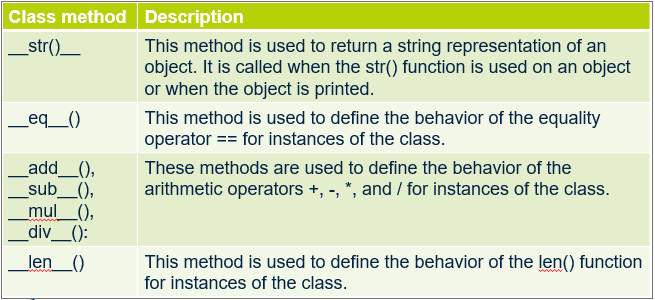
\includegraphics[scale=0.7]{special-classes.png}
	\end{center}

	\subsection*{Encapsulation:}
	Classes bundle together related data and methods that can operate on the data. The classes also allow the implementation of details to be hidden from the outside world. The internal details of the class can be changed without affecting the code that uses the class, as long the the public facing section remains the same. The process of bundling together data and methods that operate on the data, whilst hiding the method. This is called encapsulation.\\
	Encapsulation is the practice of controlling the security and access to the internal data and methods of the class. This can be achieved with access modifiers such as Public, Private or Protected. 
	\begin{itemize}
		\item Public: Class member are accessible from anywhere
		\item Private: Class members are only accessible within the class
		\item Protected: Modifier is related to subclasses (Not covered in COIT11222)
	\end{itemize}\hfill\break
	In python, unlike other languages, there is no strict access modifiers. The convention is to use underscores (\_) to indicated the intended accessibility of the attribute or method. The double indicates that the attribute or method is intended to be private. If the it does not have \_, it can be considered public. It is important to note that python does not enforce such ruling within the interpreter, they only communicate to other developers the intended accessibility.
	
	\subsection*{Getter \& Setter Methods:}
	Getter methods are used to get the value of private class attributes, whilst the setter methods set values. They are used to enforce data integrity, ensuring that only valid data is stored in the object's attributes. By using these, it prevents unwanted modifications to the attributes.

	\section*{Week 7 - Strings|Sorting|Searching:}
	\subsection*{Traversel:}
	Traversal refers to the process of capturing and computing all elements in a data structure. It involves iterating over each element individually and performing an operation or action on each one.
	\begin{multicols}{2}
		\noindent
		\texttt{ix = 0}\\
		\texttt{while ix < len(fruit):}\\
		\hspace{1em}\texttt{print(fruit[ix])}\\
		\hspace{1em}\texttt{ix += 1}\\

		\columnbreak
		A simpler way would be to use a for loop.\\
		\texttt{for i in fruit:}\\
		\hspace{1em}\texttt{print(i)}
	\end{multicols}
	
	\subsection*{String Comparison:}
	The comparison orperator (==) in python checks if two values reference the name memory location. However when comparing immutable objects like strings, is uses lexicographical order. This is based upon Unicode code point values of the specific characters in strings. The psuedocode for lexicographical oredr consists of the following:
	\begin{itemize}
		\item Compare the first character of both strings
		\item If they are both the same move to the next character
		\item If all characters in the strings match, the strings are considered to be equal
	\end{itemize}

	\subsection*{String Formatting:}
	In python there are many different way of formatting variables into strings:
	\begin{enumerate}
		\item Old-style (\%) - "My name is \%s." %name
		\begin{center}
			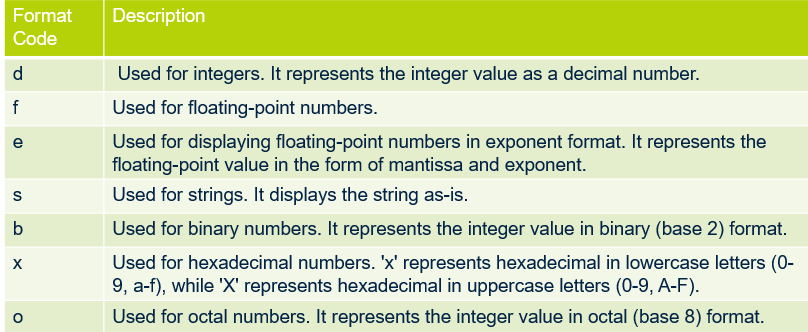
\includegraphics[scale=0.5]{format-code.png}
		\end{center}
		\item format() - "My name is \{\}.".format(name). The syntax for the \{\} is \{:[index]:[alignment][width][.precision][type(from table above)]\}
		\begin{itemize}
			\item < - Left alignment
			\item \^{\;} - Center alignment
			\item > - Right alignment
		\end{itemize}
		\item f - f"My name is {name}."
	\end{enumerate}

	\subsection*{Sorting:}
	In the contex of programming, sorting involves rearranging elements in a sequence according to a predetermined order. The order can be any way such as ascending, descending, alphabetical, etc. The reason for this sort of this is for game scoring, leaderboards, or just a generalized need for sorting.\\
	There are several different types of sorting algorithms:
	\begin{itemize}
		\item Bubble
		\item Selection
		\item Insertion
		\item Merge
		\item Quick
		\item Heap
		\item Radix
	\end{itemize}
	\subsubsection*{Selection Sort}
	For this subject only this sorting algorithm is will identified. This sorting algorithm repeatedly selects the smallest (or largest) element from an unsorted portion of the list and swaps with the element of at the beginning of the unsorted portion. The pseudocode for this algorithm is:\\
	\texttt{n = len(lst):}\\
	\texttt{for i in range(n-1):}\\
		\hspace{2em}\texttt{min\_index = i}\\
		\hspace{2em}\texttt{for j in range(i, n):}\\
			\hspace{4em}\texttt{if lst[min\_index] > lst[j]:}\\
				\hspace{6em}\texttt{min\_index = j}\\
			\hspace{4em}\texttt{end if}\\
		\hspace{2em}\texttt{end for}\\
		\hspace{2em}\texttt{swap(lst, i, min\_index)}\\
	\texttt{end for}
	\hfill\break\break
	Whilst this pseudocode applies numbers, a similar idea applies to words (letters), colours or anything else that can be sorted.

	\subsection*{Searching:}
	\subsubsection*{Linear}
	Linear searching is simple search algorithm that sequentially checks each element in a collection against a target value. It continues linearlly through the collection through until the element is found or the whole collection is sorted. The pseudocode for this is:\\
	\texttt{def linear\_search(lst, target):}\\
		\hspace{2em}\texttt{n = len(lst)}\\
		\hspace{2em}\texttt{index = -1}\\
		\hspace{2em}\texttt{for i in range(n):}\\
			\hspace{4em}\texttt{if lst[i] == target:}\\
				\hspace{6em}\texttt{index = i}\\
				\hspace{6em}\texttt{break}\\
			\hspace{4em}\texttt{end if}\\
		\hspace{2em}\texttt{end for}\\
		\hspace{2em}\texttt{return index}
	\hfill\break\break
	\subsubsection*{Binary Search}
	Binary search, searches by halves (A.K.A divide and conquer). It requires the list to already be sorted. The pseudocode for this search is:\\
	\texttt{def binary\_search(lst, target):}\\
		\hspace{2em}\texttt{index = -1}\\
		\hspace{2em}\texttt{left = 0}\\
		\hspace{2em}\texttt{right = len(lst) - 1}\\
		\hspace{2em}\texttt{while left <= right:}\\
		\hspace{4em}\texttt{mid = (left + right)//2}\\
			\hspace{4em}\texttt{if lst[mid] == target:}\\
				\hspace{6em}\texttt{index = mid}\\
				\hspace{6em}\texttt{break}\\
			\hspace{4em}\texttt{elif lst[mid] < target:}\\
				\hspace{6em}\texttt{left = mid + 1}\\
			\hspace{4em}\texttt{else:}\\
				\hspace{6em}\texttt{right = mid - 1}\\
			\hspace{4em}\texttt{end if}\\
		\hspace{2em}\texttt{end while}\\
		\hspace{2em}\texttt{return index}
	\hfill\break\break

	\section*{Week 8 - Working with Files:}
	\subsection*{Lists:}
	\subsubsection*{Aliasing}
	Just recall that when to objects are referencing the same mutable item. Changing one, will affect the other. To check whether objects are referencing the same memory location use the is modifier. e.g. a is b, will return true if they reference the same location. It is only refered to as aliasing if the variable names are different. Aliasing is only a problem, and cause unexpected errors on mutable objects like lists. If they are aliased to a immutable object this will not work, because python creates a new location for each mutable object.
	\subsubsection*{Cloning Lists}
	There are two main ways of cloning a list.
	\begin{enumerate}
		\item Slicing:\hfill\break
			a = [1, 2, 3]\\
			b = a[:] \# b is now [1, 2, 3]
		\item The list() constructor:\hfill\break
			a = [4, 5, 6]\\
			b = list(a) \# Converts a into a list \\
			a is b \# Now False\\
			print(b) \# [4, 5, 6]
	\end{enumerate}

	\subsection*{Strings to Lists:}
	It is possible to convert each word in a sentence to an item in a list. To do this a split() function is used. The item specified in the () will be used to split the string and not appear in the list, e.g. () will split on the spaces, or ('ai') will spilt on the letters ai.\\
	It is also possible to join together a list with the join() function. This uses a "glue" that will be placed between the items. 

	\subsection*{Working with Files:}
	For python to have access to any files on a system within a program, it must open the file. Python just uses the open() functions. Within this there are a number of different parameters that must be understood for specific file types that can be opened, see image below. It is also important to remember to close the file handle after working with the file is completed.
	\begin{center}
		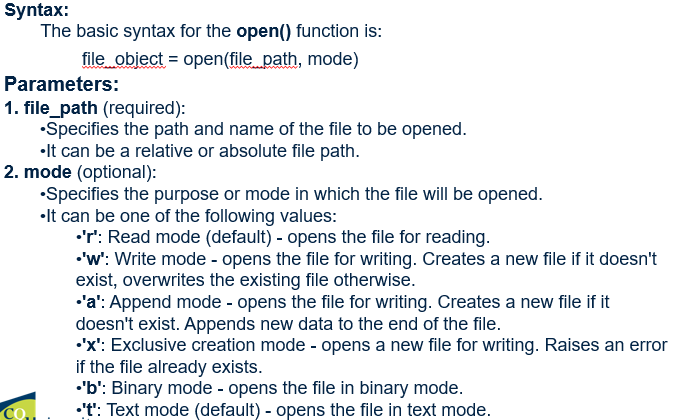
\includegraphics[scale=0.75]{open-para.png}
	\end{center}
	To read a line in the file the readline() or to read the entire file the readlines() can be used. The .strip() can be used to get rid of the newline (\textbackslash n) characters in a file.

	\section*{Week 9 - Exception Handling:}
	Exception handling allows parts of the program to fail gracefully. These include the classic divisio by zero (ZeroDivisionError), item not existing (IndexError), of changing something to a different data type (TypeError). It dose this through a try except program. The exception statement follows the type of the error that is being excepeted, these can include custom exceptions. The finally clause will also execute even if try part is successful or fails.\\
	Custom exceptions can be raised at any time and block the code in the try section from running and go the the exceptio MyException.
\end{multicols}
\pagebreak
\begin{center}
	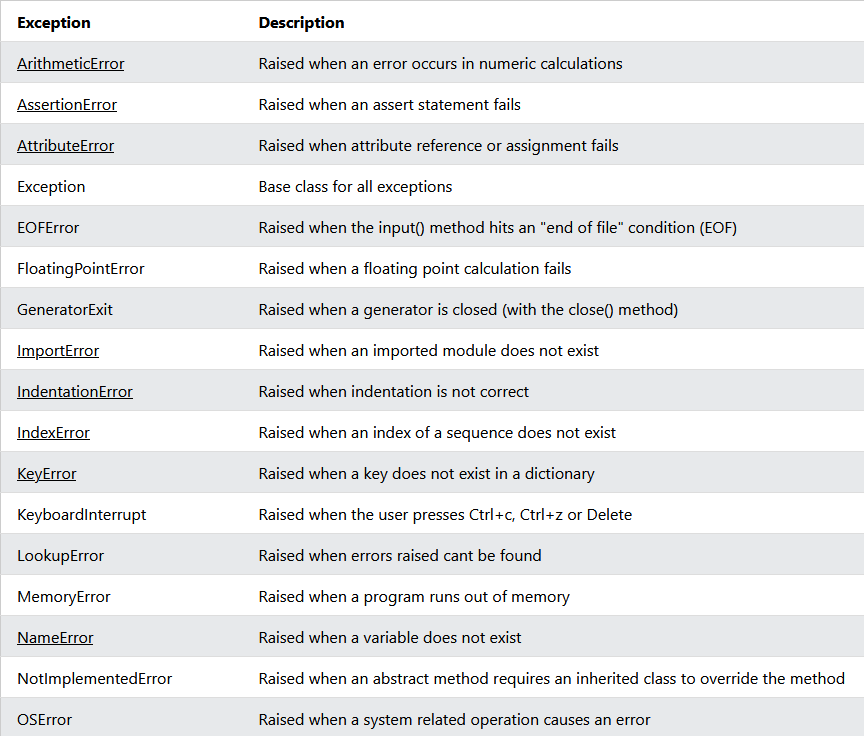
\includegraphics[scale=0.7]{errors-1.png}
	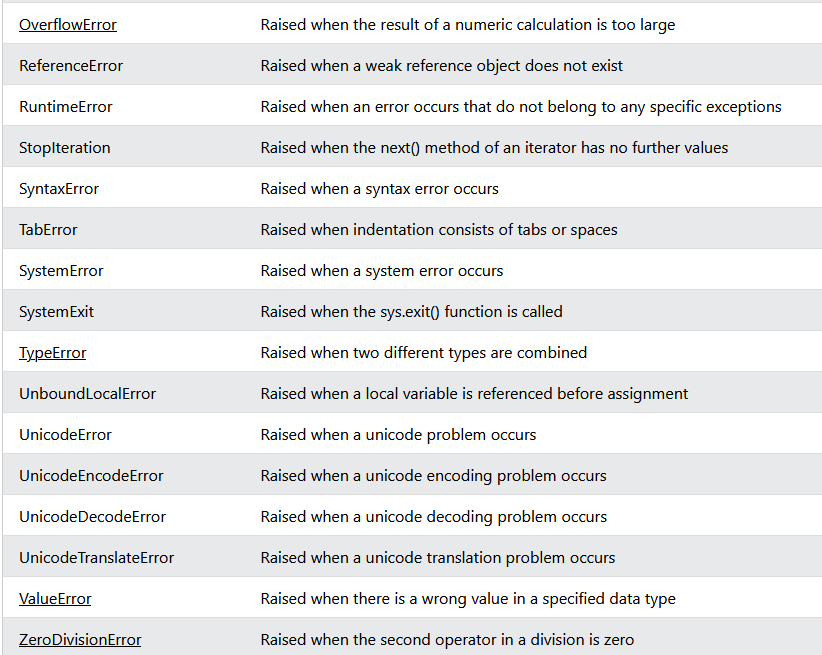
\includegraphics[scale=0.7]{errors-2.png}
\end{center}
\end{flushleft}
\end{document}
